\section{Design}\label{Design}
    [The actual design of our implementation.]
    \subsection{Client Side}\label{Client Side}
        [The client side design.]
        \subsubsection{Data Flow}\label{Data Flow}
        [how the data moves through the client.]
            \begin{figure}[h]
            \centering
            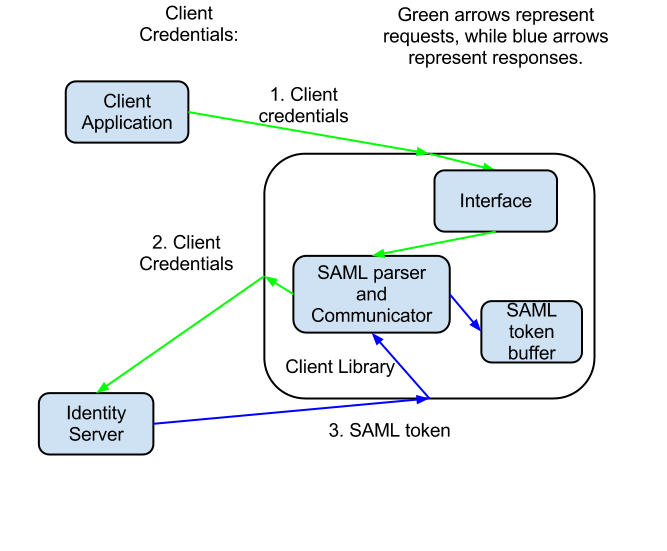
\includegraphics[scale=0.5]{ClientCredentialsDataFlowDiagram}
            \caption{Client Data Flow}
            How data flows on the client side.
            \label{fig:ClientCredentialsDataFlowDiagram}
        \end{figure}
        
        \begin{figure}[h]
            \centering
            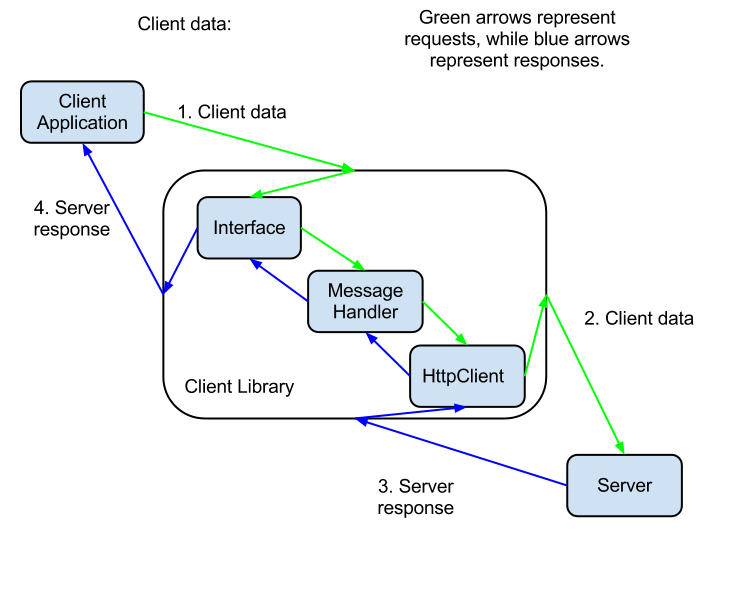
\includegraphics[scale=0.5]{ClientDataFlowDiagram}
            \caption{Client Credentials Flow}
            The flow of the credentials to and in the client side.
            \label{fig:ClientDataFlowDiagram}
        \end{figure}
        
    \subsection{Server Side Design}\label{Server Side Design}
        [The server side design specifics.]
        \subsubsection{SAML Authentication}\label{SAML Authentication}
            [The SAML authentication flow. How the request and authentication actualle happens.]
            \begin{figure}[h]
                \centering
                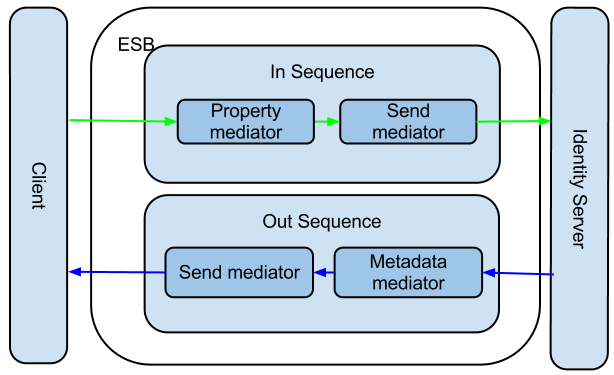
\includegraphics[scale=0.5]{SAMLauthenticationflow}
                \caption{SAML Authentication Flow}
                \label{fig:SAMLauthenticationflow}
            \end{figure}
        
        \subsubsection{Data Flow}\label{serverdataflow}
            [How the data moves on the server side of our application.]
            \begin{figure}[h]
                \centering
                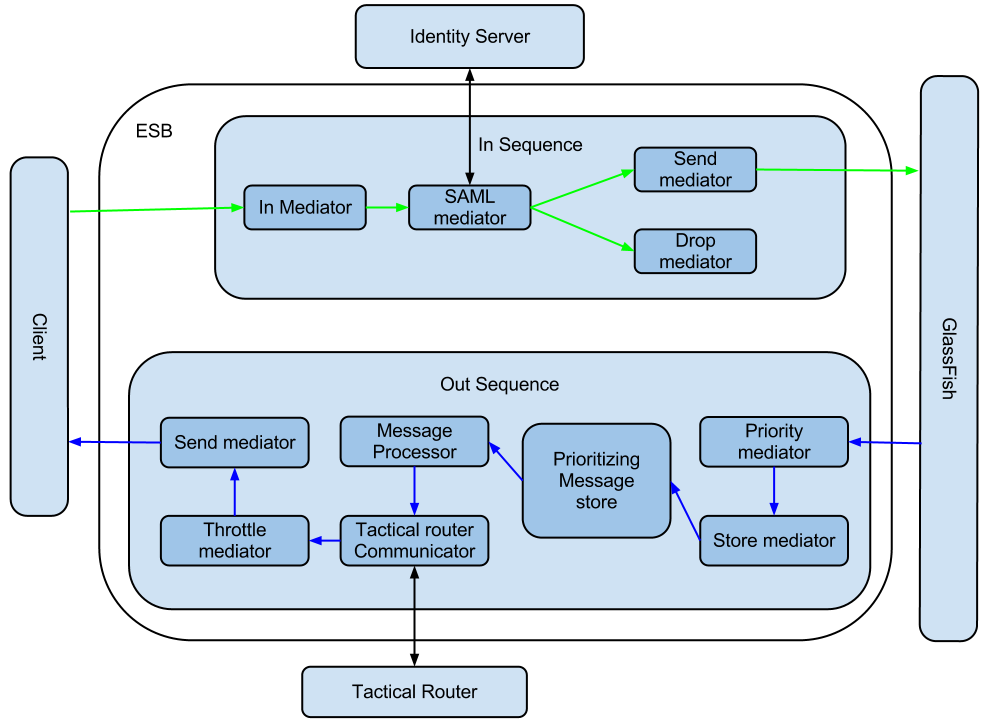
\includegraphics[scale=0.4]{DataFlowDiagramServer}
                \caption{Server Data Flow}
                \label{fig:serverDataFlow}
            \end{figure}

